调用普通函数(或过程)时,然后运行到它们的结束(或直到到达返回语句或抛出异常),而协程是可以分多个步骤运行的函数(参见图14.1)。

某些时刻,可以挂起一个协程,所以该函数暂停其计算,直到恢复。挂起可能是因为函数必须等待某些东西,有其他(更重要的)事情要做,或者有一个中间结果要给调用者。

因此,启动协程意味着启动另一个函数,直到它的一部分完成。调用函数和协程都在它们的两条执行路径之间来回切换。注意,这两个函数不是并行运行的,我们用控制流来打乒乓球:

\begin{itemize}
\item 
函数可以通过开始或继续协程的语句来决定启动或恢复其当前控制流。

\item 
当协程运行时,协程可以决定挂起或结束其执行,启动或恢复协程的函数将继续执行其控制流。
\end{itemize}

协程的最简单形式中,主控制流和协程的控制流都在同一个线程中运行。不需要使用多线程,也不需要处理并发访问,但可以在不同的线程中运行协程。甚至可以在不同的线程上将协程恢复到先前挂起的位置。协程有一种正交特性,但其可以与多个线程一起使用。甚至可以在不同的线程上将协程恢复到先前挂起的位置。

\begin{center}
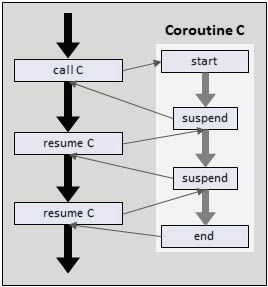
\includegraphics[width=0.4\textwidth]{content/chapter14/images/1.png}\\
图14.1 协程
\end{center}

实际上,使用协程就像在后台有一个函数,你可以不时地启动和继续。然而,由于协程的生命周期超出了嵌套作用域,因此协程也是一个将其状态存储在某些内存中并提供处理状态的API的对象。

C++中有几个关于协程的基础工具:

\begin{itemize}
\item 
只需在函数中使用以下关键字之一即可隐式定义协程:

\begin{itemize}
\item 
co\_await

\item 
co\_yield

\item 
co\_return
\end{itemize}

若这些关键字在协程中都不需要,则必须显式地使用co\_return;语句。

\item 
协程通常返回一个对象,作为调用者的协程接口。根据协程的目的和用途,该对象可以表示一个不时挂起或切换上下文的正在运行的任务,不时产生值的生成器,或者一个按需惰性地返回一个或多个值的工厂。

\item 
协程无堆栈。不挂起外部协程的情况下,无法挂起在外部协程中调用的内部协程,只能将外部协程作为一个整体挂起。

当协程挂起时,协程的状态作为一个整体被存储在与堆栈分开的对象中,以便它可以在完全不同的上下文中(在不同的调用堆栈中,在另一个线程中等)恢复。
\end{itemize}












